\chapter{Deep Learning}
\section{Methods}

\begin{enumerate}
\item Image 2 Image, limited angle / limited dose
\item Sino 2 Sino
\item Poly 2 Mono
\item GAN???
\end{enumerate}

Here will be n outline of what is to come in this section

\subsection{U-Net Architecture}

In this section the structure of the U-Net architecture will be described. This network structure is used with variations for all the models which follow. The underlying 
structure is based on the standard architecture used in classification problems with the addition of an expansive path which upsamples the features. There exist similarities 
with the structure found in autoencoders. The initial half of the network can be thought of as an encoding structure followed by a decoding structure in the second half. In contrast
to the usual compressive nature of an autoencoder the U-Net downsamples the image dimension but increases the number of channels and so in the centre of the architecture there is 
not a decrease in the number of features. A schematic of the network can be seen in figure \ref{UNet}. 

The first half of the network is structured in the following way;

\begin{itemize}
    \item Stage 1: Input image of size $256 \times 256 \times 1$ is passed through three layers of $3 \times 3 \times 64$ padded convolutions resulting in an output of
    size $256 \times 256 \times 64$. Before each layer instance normalisation is applied and following each layer the output is passed through a ReLU activation 
    function. After the three convolution layers a $2 \times 2$ max pooling operation is applied in order to downsample the image by a factor of two resulting in an output 
    of size $128 \times 128 \times 64$.
    \item Stages 2-4 : Each stage consists of 2 layers of $3 \times 3 \times k$ padded convolutions, such that $k$ doubles at each stage. Instance normalisation is applied before
    each layer and ReLU activation is applied after each layer. The final layer in each stage is $2 \times 2$ max pooling operation. After stage four the output is of size $32 \times 32 \times 512$.  
    \item Stage 5 : The same as in stages 2-4 without a final max pool layer. The resulting output size is $16 \times 16 \times 1024$.
\end{itemize} 

In a standard classification network the above would be followed by a fully connected layer which would be used to give class probabilities. However in the U-Net a symmetric
expansive path is now added. The second half of the network is structured as follows;

\begin{itemize}
    \item Stage 1 : A transposed convolution layer is now applied to upsample the image to be of size $32 \times 32 \times 1024$. Instance normalisation is then applied followed
    by skip connecting via concatenation of the output with the corresponding output from stage 4 of the first half of network resulting in an output of size $32 \times 32 \times 1024 + 512$. This is now followed by 2 layers
    of standard padded $3 \times 3 \times 512$ convolutions. Instance normalisation is applied before each layer and ReLU activation is applied after each layer.
    \item Stage 2-4 : Each stage begins with an upsampling transposed convolution followed by a skip concatenation from the corresponding stage of the first half of the network. This is followed by 
    two layers of standard convolutions. Instance normalisation is applied before each layer and ReLU activation is applied after each layer. At the end of stage four the output
    is of size  $256 \times 256 \times 64$.
    \item Stage 5 : The final stage of the network is a $1 \times 1 \times 1$ convolution layer without a nonlinearity applied. The final output is of size $256 \times 256 \times 1$ matching the 
    initial network input size.
\end{itemize}

The various models in the next sections have slight variations on the above structure, mainly focused on the final stage of the second half of the network, which will be described below. All networks are however 
trained using Adam optimisation algorithm with a simple least squares loss between network outputs and target.  

\subsection{Sparse Angle reconstruction - Image Domain}

In this model the aim is to train the network to learn a mapping between reconstructions with sparse angular projections and reconstructions with more densely sampled angular
projections. The data used to train this network consists of five hundred pairs of FBP reconstructions, along with a validation set of one hundred pairs and a test set of a further 
five hundred image pairs. Each training sample given to the network $(x_i,y_i)$ such that $x_i,y_i \in \mathbb{R}^{256 \times 256 \times 1}$, where $x_i$ is the input a sparsely sampled
reconstruction and $y_i$ is the target a densely sampled reconstruction. Samples are passed into the network one at a time with weight update applied after each sample. 

Three training sets were constructed which had successively sparser angular sampling. The first set consisted of reconstructions calculated, using ODL, from fifty projections equally spaced 
between $0$ and $2 \pi$ radians consisting of five hundred detector elements. The second and third had twenty and ten equally spaced projections respectively. Examples of training pairs can be seen in
figures \ref{trainingsamples1}, \ref{trainingsamples2} and \ref{trainingsamples3}. The projections were calculated based on a simulated phantom consisting of two materials. A main square region made of one 
material with a series of random circular regions of various sizes and locations. Materials used were not chosen with any physical properties in mind. Projections were implemented using Astra's 
parallel geometry projection operator on the GPU.

\begin{figure}[htb]
\centering
     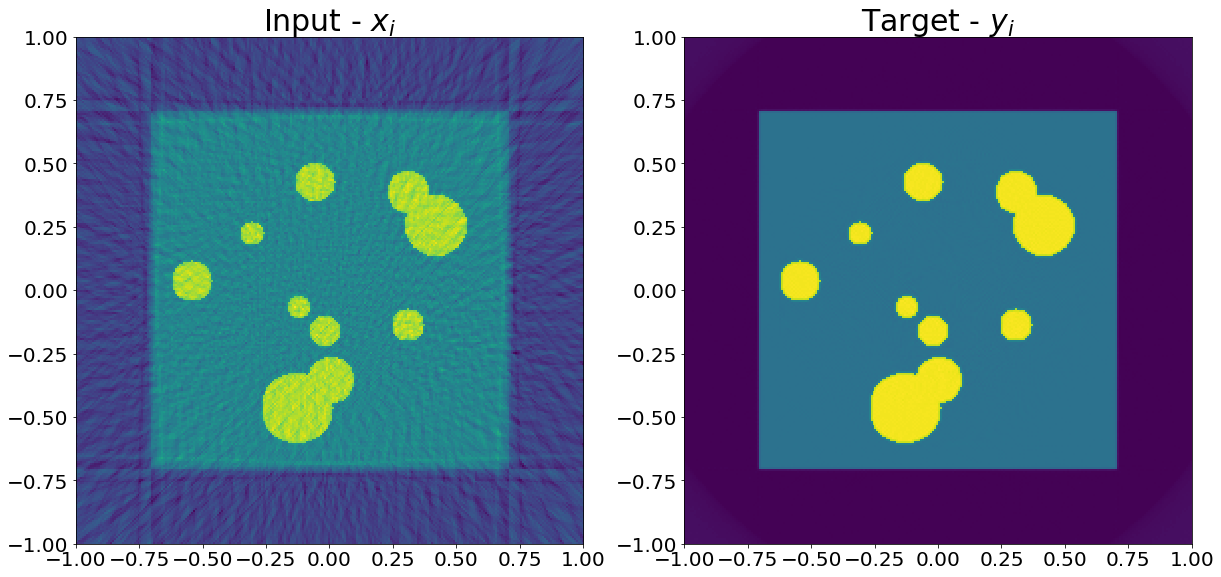
\includegraphics[width=\textwidth]{figures/trainingsamples1} \
  \caption{Training sample: fifty projections input and one thousand projections target}
  \label{trainingsamples1}
\end{figure}

\begin{figure}[htb]
\centering
     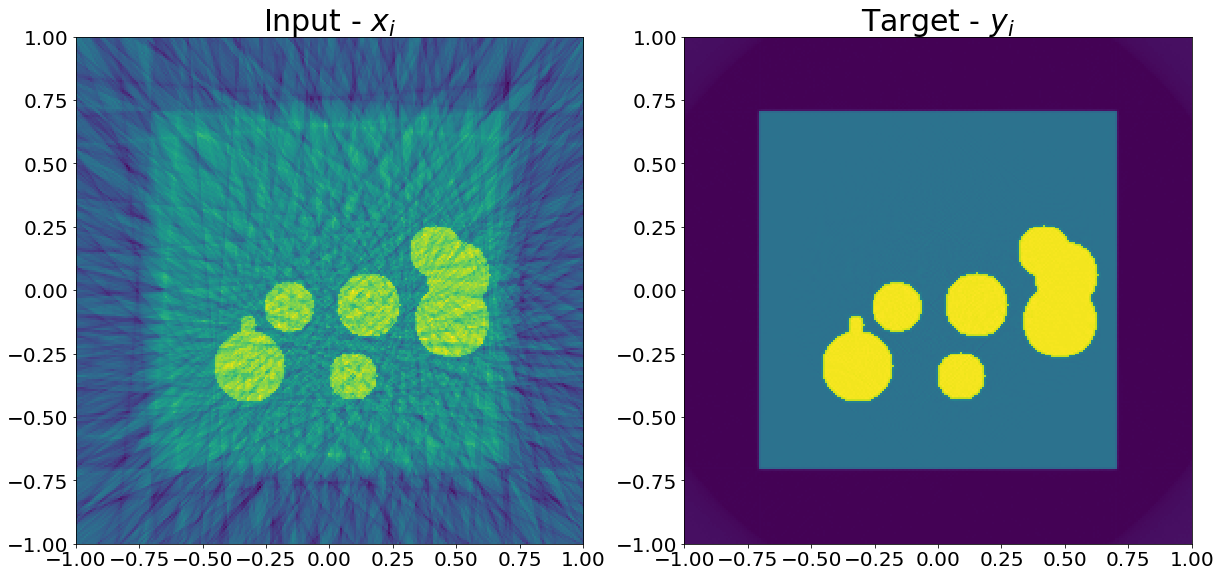
\includegraphics[width=\textwidth]{figures/trainingsamples2} \
  \caption{Training sample: twenty projections input and one thousand projections target}
  \label{trainingsamples2}
\end{figure}

\begin{figure}[htb]
\centering
     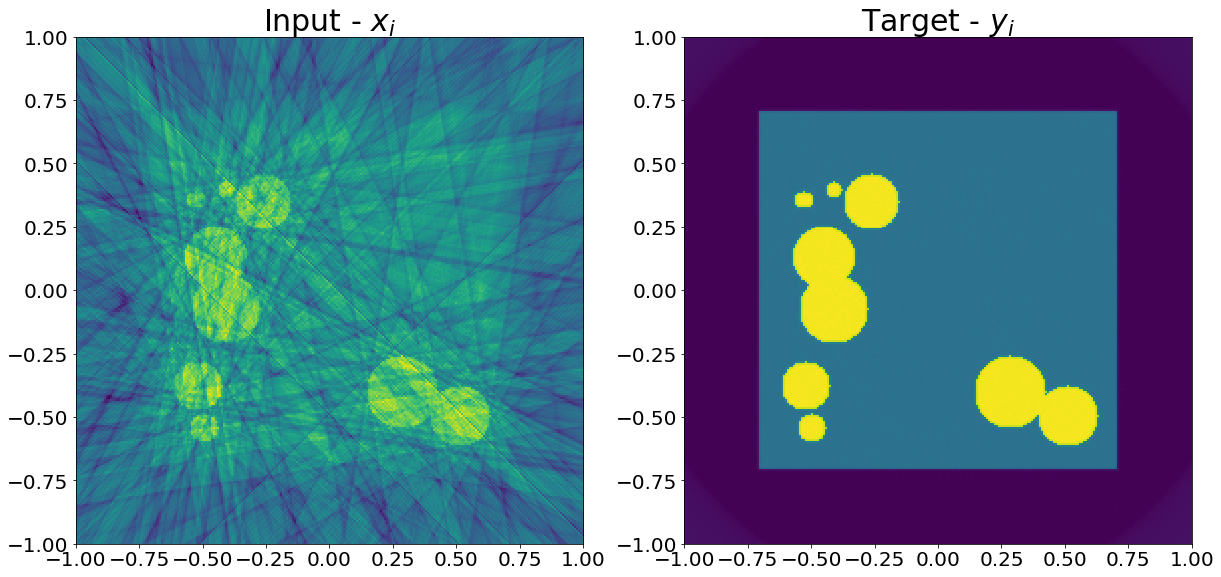
\includegraphics[width=\textwidth]{figures/trainingsamples3} \
  \caption{Training sample: ten projections input and one thousand projections target}
  \label{trainingsamples3}
\end{figure}

The U-Net architecture previously described was used with the addition of a final skip connection connecting the input layer to the output layer. This connection is not a concatenation as used in 
lower layers but instead the input image is added elementwise to the output of the network. This means that the network is not trying to learn a direct mapping but is instead trying to learn the structure 
of the negative residual, the noise, between input and label. 

The model was trained over ten epochs, full cycles through all training data, using the Adam optimisation algorithm with a fixed learning rate of $0.001$.

\subsection{Sparse Angle reconstruction - Projection Domain}

In this section a model with a similar goal as above will be described. The main difference will be that the network will work in the projection, or sinogram, domain rather
than in the image domain. The U-Net architecture will be used to learn a mapping from sparsely sampled sinograms to more densely sampled output sinograms. The training data 
for this model was again constructed using the same phantom as previously described. Now the training samples $(x_i,y_i)$ are such that $x_i,y_i \in \mathbb{R}^{256 \times 256 \times 1}$. 
The input to the network $x_i$ will be a zero padded ${256 \times 256 \times 1}$ sinogram, whilst the target $y_i$ will be a densely sampled sinogram. These samples were 
constructed by calculating projections at $512$ equally spaced angles between $0$ and $2 \pi$ radians, this is the target, and then removing all projections apart from every
$k^{th}$ for $k=8, 16, 32, 64$. The projections were calculated using Astra's parallel geometry projection operator on the GPU. Examples of these training samples can 
be seen in figures \ref{trainingsamples4}, \ref{trainingsamples5}, \ref{trainingsamples6} and \ref{trainingsamples7}.

\begin{figure}[htb]
\centering
     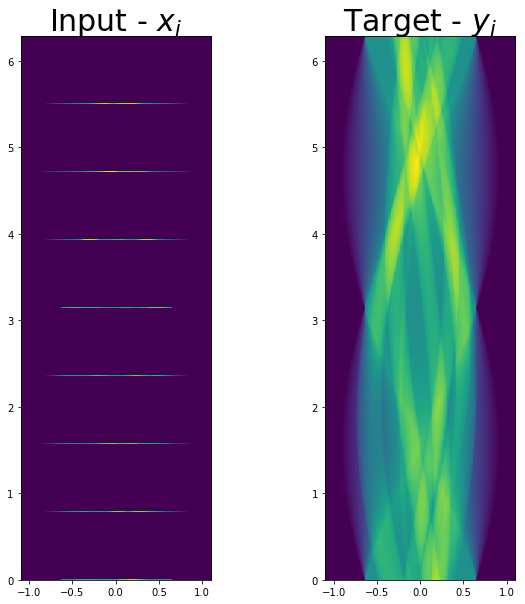
\includegraphics[width= 0.7 \textwidth]{figures/trainingsamples4} \
  \caption{Training sample: every $64^{th}$ projection kept for input and $512$ projections for target}
  \label{trainingsamples4}
\end{figure}

\begin{figure}[htb]
\centering
     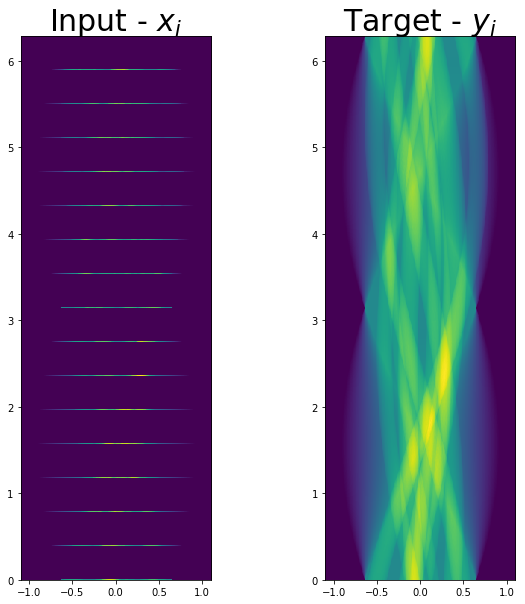
\includegraphics[width=0.7 \textwidth]{figures/trainingsamples5} \
  \caption{Training sample: every $32^{nd}$ projection kept for input and $512$ projections for target}
  \label{trainingsamples5}
\end{figure}

\begin{figure}[htb]
\centering
     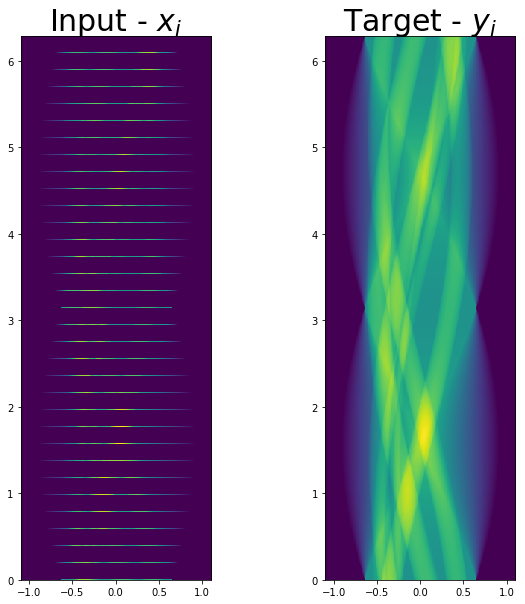
\includegraphics[width=0.7 \textwidth]{figures/trainingsamples6} \
  \caption{Training sample: every $16^{th}$ projection kept for input and $512$ projections for target}
  \label{trainingsamples6}
\end{figure}

\begin{figure}[htb]
\centering
     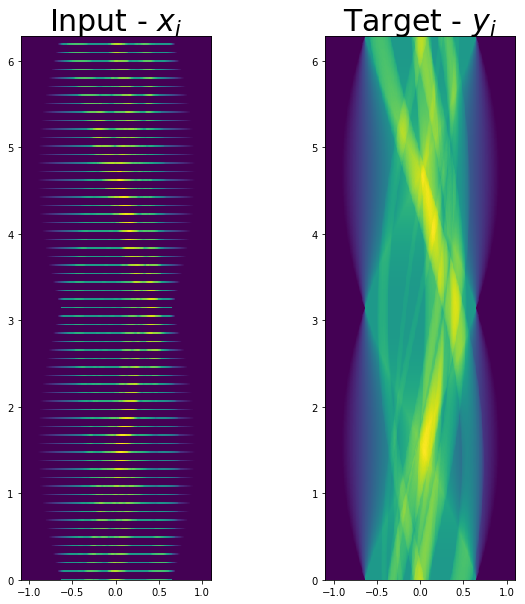
\includegraphics[width=0.7 \textwidth]{figures/trainingsamples7} \
  \caption{Training sample: every $8^{th}$ projection kept for input and $512$ projections for target}
  \label{trainingsamples7}
\end{figure}

For this model it was necessary to make some alteration to the transposed convolution layers due to the non-square nature of the input, other than this alteration the model 
is the same as described above. Again the network was attempting to learn a mapping from the input to the residual, the output of the network should be what is needed to add elementwise
to the input to obtain the target. This is essentially the task of imputing the missing projections. 

As above this model was trained over ten epochs using the Adam optimisation algorithm with a fixed learning rate of $0.001$.

\subsection{Polychromatic Artefact removal}


Lorem ipsum dolor sit amet, consectetur adipiscing elit. Pellentesque laoreet maximus ex, ac rutrum nibh porta sit amet. Fusce fringilla neque in vulputate bibendum. In accumsan sapien velit, vitae interdum augue ullamcorper eget. Proin eu elit neque. Curabitur convallis sed dui in posuere. Nulla nec volutpat urna, a scelerisque nulla. Praesent viverra nisl purus, eu ullamcorper ex lacinia viverra. Maecenas viverra, ex ac sollicitudin elementum, purus enim vehicula leo, non faucibus elit metus ut odio. In et elit arcu. Duis eu scelerisque lacus. Nulla quis nunc pretium, sagittis leo in, vestibulum massa. Integer vulputate quam turpis, vitae bibendum quam rhoncus quis. Integer mollis leo nec est convallis tempus. Nunc a imperdiet massa. Donec sit amet rhoncus lacus, eu semper eros. Fusce bibendum maximus finibus.

Duis quis sapien convallis, viverra libero sed, ultrices tortor. Pellentesque turpis erat, posuere in eros vitae, ullamcorper accumsan massa. Donec justo nibh, maximus vel maximus quis, aliquet in tellus. Aliquam viverra suscipit ultricies. In tortor metus, maximus sed nulla ornare, bibendum mattis enim. Duis eu tortor tempor quam tincidunt semper id tempor sapien. Morbi est massa, maximus quis lacus ac, tincidunt vulputate urna. Nulla facilisi. Etiam aliquet consectetur mi et mollis. Praesent faucibus iaculis ultricies. Ut suscipit felis eros, eget sagittis nunc sollicitudin in. Phasellus interdum quam magna, at vulputate tortor pulvinar sit amet. Aenean pulvinar velit vel malesuada dictum. Donec congue fermentum metus, sit amet ultricies nunc rhoncus ut.

Nam pulvinar, augue et semper pretium, tellus tortor mollis orci, sit amet cursus neque nunc nec purus. Proin at vehicula libero, auctor aliquet orci. Duis congue sagittis malesuada. Curabitur pharetra, nulla eu bibendum sagittis, urna quam pharetra dui, eu lobortis dui urna ac ante. Donec id blandit nunc. Donec maximus magna nec enim dignissim dapibus. Nulla at orci vitae tortor eleifend hendrerit. Pellentesque consequat nunc eget sem varius, dapibus malesuada orci feugiat. Nunc sed arcu id elit maximus commodo. Integer vel tellus non lacus elementum scelerisque et sed elit. Proin sagittis risus eget tortor sagittis pharetra. Vestibulum porta neque eget sapien auctor, id porttitor libero accumsan. Aliquam erat volutpat. Duis vel varius diam. Fusce non neque sed ante scelerisque laoreet. Maecenas tempus lorem ac sem rutrum, ac consequat nisl congue.

Vivamus quis blandit nisl. Vestibulum interdum nisl nec blandit aliquam. Etiam dignissim, ex et facilisis maximus, quam enim vestibulum ipsum, ac rutrum mauris dolor non lacus. Aliquam ac euismod mi, dictum tempus lectus. Fusce a risus vehicula, vulputate enim at, dictum magna. Aliquam ultricies nec libero a fringilla. Praesent sed neque dapibus risus facilisis dignissim in eu velit. Vestibulum libero tortor, ultrices vel diam aliquam, tincidunt feugiat dolor. Donec quis laoreet velit, a pellentesque diam. Mauris a pellentesque metus. Proin at tristique mi, pulvinar suscipit dolor.

Vestibulum sollicitudin interdum porttitor. Donec facilisis turpis in vestibulum ultrices. Morbi erat diam, pharetra nec lectus sed, scelerisque accumsan augue. Morbi aliquam dui nec urna auctor pretium. Pellentesque eu dignissim ante. Nulla imperdiet diam at odio auctor scelerisque. Aliquam erat volutpat. Lorem ipsum dolor sit amet, consectetur adipiscing elit. Sed bibendum, tellus nec gravida sagittis, lacus mi fermentum neque, at finibus risus ipsum at ante.

Pellentesque rutrum urna accumsan ligula ultricies ornare. Nulla sollicitudin nibh vitae odio dignissim suscipit. Fusce aliquam posuere consectetur. Sed sit amet congue elit, quis aliquam purus. Sed dolor eros, molestie sit amet scelerisque tempus, consequat at nibh. Suspendisse faucibus nibh ut leo placerat, eu suscipit lorem malesuada. Vivamus eleifend vulputate ante. Ut et viverra arcu. Phasellus rutrum in elit sit amet fringilla. Vestibulum vestibulum magna ut tincidunt ultrices. Aliquam eu nibh sed nunc tristique finibus et id ex.

Nam eget dolor condimentum nisl aliquet rutrum. Integer volutpat, mauris in ullamcorper rutrum, sapien ligula euismod urna, ac scelerisque eros ipsum at nulla. Vestibulum auctor suscipit facilisis. Vivamus pharetra eget est at pulvinar. Aenean facilisis consequat orci vel tincidunt. Duis vitae leo mauris. Nunc laoreet molestie nulla et molestie. Etiam gravida tempus laoreet. Vivamus at eros molestie, semper ex in, pulvinar neque. In quam ex, placerat ac ipsum sit amet, pretium bibendum eros. Duis feugiat laoreet diam, a rhoncus tellus dignissim quis. Suspendisse pretium, sapien sed fringilla aliquam, mauris nisl elementum tortor, a feugiat leo nisl nec ipsum. Suspendisse orci mi, luctus in rutrum in, pulvinar sit amet tortor. Morbi suscipit arcu arcu, eu consequat metus tempus vel. Praesent convallis, orci et finibus euismod, magna odio ornare ligula, sed congue erat ipsum quis lacus.

Fusce ut fringilla ante. Etiam ac interdum dui. Curabitur mattis ac tellus non tempus. Pellentesque et ex vitae felis dapibus cursus. Aliquam erat.